\section{Interest flooding mitigation methods}
\label{sec:design}

% Points what should be here:
% - What can be done (in general) to mitigate flooding attack
% - Which building blocks NDN architecture gives to mitigate Interest flooding attacks: Interest limits, ability to measure Interest satisfaction performance (Interest satisfaction stats)
% - Methods to set these limits: static/dynamic
% - Methods how limits can be applied: best-effort (fifo), "fair" queuing, probabilistic
% - Reference to caching: we don't consider it here, but caching provides additional level of protection, especially for certain types of attacks

% Our definition of attack mitigation is that good clients are still able to access data on the producer.

In this section we present several methods to mitigate Interest flooding attacks in NDN, featuring different degrees of implementation complexity, as well as different degrees of effectiveness.

%   - Naive approach to Interest Limits (that is called physical limits everywhere else)
%     Example how this can be implemented in a simple way
%     Baseline solution
%   - Interest limits with "fair" queuing
%     Improving problem of simple limits (no single face can dominate), but doesn't solve the proble

% - Attack mitigation
%   - Per-incoming interface Interest statistics

%   - Dynamic Interests limit adjustments

%   - Probabilistic Interest accept

Our methods to mitigate Interest flooding attack rely on the fundamental principle of the NDN architecture: the flow balance between Interest and Data packets: one Interest packet (the only communication initiator) can be satisfied with at most one Data packet.
Because NDN is host-to-host architecture (as opposed to end-to-end in the current IP Internet), the flow balance principle allow any entity on the network, end-hosts and routers, control what and how much Data they want to receive.
Therefore, any node can limit the number of forwarded Interests, effectively limiting the amount of the retrieved Data.
At the same time, each forwarded Interest can be used to build up various data plane performance statistics, such as per-incoming interface ratios of satisfied Interests.

\subsection{Na\"{i}ve attack mitigation}

% In a normal network operation, the size of Interests packets is supposed to be significantly smaller than the size of the requested Data.

% All communication in NDN network is host-to-host and receiver-driven.

The most obvious and na\"{i}ve method to mitigate the Interest flooding attack is to limit the number of forwarded Interests out of each interface. 
That is, if it is known that the amount of already requested data ($=$~amount of forwarded Interests) can fully utilize the downstream link, an NDN node---either an end-user or an NDN router---has absolutely no point in forwarding new incoming Interests and creating corresponding PIT entries.
For example, if a router A on Fig.~\ref{fig:flooding example} already forwarded 125 Interests requesting 1000-byte Data packets, any new incoming Interests can be almost safely dropped, provided the link capacity between A--B is 100~Mbps and delay is 10~ms.
In other words, 125 Data packets returned by router B will fully utilize the link ($125 \times 1000 \mathrm{~bytes} \approx 10\mathrm{~ms} \times 100\mathrm{~Mbps}$) and any excess Data would be dropped.

\subsubsection{\textbf{Interest limits (physical limits)}}
\label{sec:physical limits}

\subsection{Physical limits}
\label{sec:physical limits}

The requirement to send an Interest in order to receive Data packet, provides an NDN consumer a unique opportunity to request the right amount of Data.
Moreover, the same opportunity to control the amount of data flow is given not only to consumers, but all routers between consumer and producer (or nearby caches).  
In other words, every node, either a consumer or an intermediate router, is able to control how much data it wants to receive by limiting the number of forwarded Interests.

The limitation can implemented in a number of different ways, including leaky bucket scheduling and window-based flow control.
We decided to following TCP-like window-based flow control and applied the sliding window approach to implement Interest limits.

The size of the window defines how many Interests can be send out before Interests get satisfied or expired.
From the one hand, this size should be large enough to ``fill the pipe,'' meaning that a node needs to send enough Interests to receive Data at full capacity of the incoming link.
On the other hand, the window's size should not be too large to avoid excessive buffering and congestion of the Data packet.
Thus, the ideal size for such a window need to be defined proportional to link's bandwidth-delay product~\cite{tcp-survey}.
With the objective to request as many Data packets, as downstream link can pump through, we are getting the following equation for Interest limit:

\[
\mathrm{Interest\ Limit} = Delay\ [s] \cdot \frac{\mathrm{Bandwidth\ [Bytes/s]}}{\mathrm{Data\ packet\ size\ [Bytes]}}
\]

Note that the value of \textit{Delay} is not known a priory and varies between different Interest-Data flows.
However, we do not need to know the exact value of the delay and can set it as an average round trip delay among all flows (with a reasonable filtering of outliers).
This way, the statistical traffic multiplexing with link-level buffering will allow full utilization of the downstream link.
Exactly the same reasoning can be applied to the \textit{Data packet size} parameter, which can also be set to an average observed Data packet size.

Unlike rate-based approaches, window-based limiting does not require precise knowledge about the rate, as well does not need precise scheduling mechanisms.
Like in TCP, the window-based flow is self-clocking, easily adjusting itself to any traffic patterns.

%%% Local Variables: 
%%% mode: latex
%%% TeX-master: "../paper"
%%% End: 


%%%%%%%%%%%%%%%%%%%%%%%
%%%%%%%%%%%%%%%%%%%%%%%
%%%%%%%%%%%%%%%%%%%%%%%

\subsubsection{\textbf{Physical limits with per-interface fairness}}
\label{sec:queuing}

% \subsection{Physical limits with ``fair'' queuing}
% \label{sec:queuing}

% However, this limitation approach does not attempt to utilize data plane performance knowledge (i.e., Interest satisfaction ratio statistics) to discriminate good and malicious Interests.

To partially overcome deficiencies of the Physical limits algorithm we need to ensure that the forwarded Interests represent at least a ``fair'' mix of the Interests received from different neighbors (interfaces).
That is, if the routers A on Fig.~\ref{fig:flooding example} has a very tight token budget, these tokens should be fairly distributed between incoming interfaces \texttt{eth0} and \texttt{eth1}.
Because of the very small volume of Interests, we cannot simply rely on network buffers to do statistical multiplexing of Interests, as they would almost never be buffered.
At the same time, until bag of tokens is not empty, there is no reason to delay Interest forwarding, as we do not known how many and from which interfaces Interests will arrive in the future.
Therefore, in order to achieve the goal of ``fair'' mixing of Interests, we need to implement additional mechanisms to buffer and mix incoming Interests, only if they cannot be immediately forwarded.

For the buffering part, we can reuse Pending Interest Table, with a small extension to support flagging of the Interests that cannot be forwarded immediately (see example on Fig.~\ref{fig:queueing}). 
As for the mixing part, we need an additional fair queuing mechanism, which can be implemented in a form of hierarchical queues (on Fig.~\ref{fig:queueing})\footnote{This essentially is a class based queuing, with classes for each outgoing/incoming interface.} or using virtual time approach~\cite{zhang1990virtual}. 
It should be noted that unlike normal queuing, Interest queues do not actually store a packet, but merely a bi-directional pointer to the existing PIT entry.
This way, PIT entry can be quickly updated when the Interest is actually forwarded, as well as the element can be removed from the queue when the Interest expires.

\begin{figure}[htbp]
  \centering
  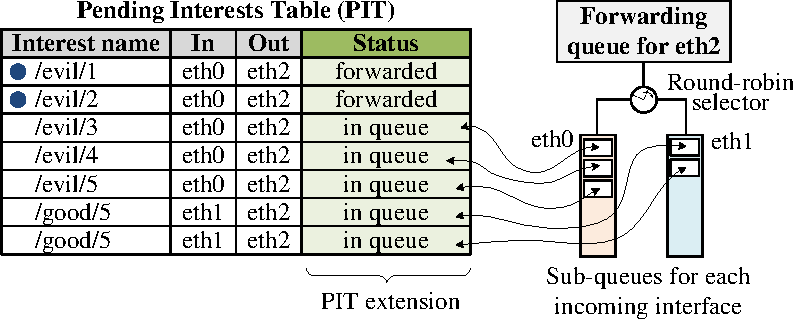
\includegraphics[scale=0.65]{queue}
  \caption{Interest queuing: if tokens are unavailable, the router creates PIT entry, but instead of forwarding, enqueued the Interest}
  \label{fig:queueing}
\end{figure}

A more formalized description of the Physical limits algorithms with per-interface fairness is presented in Pseudocode~\ref{alg:queuing}.
The algorithm extends the base Physical limits algorithm by enabling queuing when the bag of tokens is empty (lines 7--10), as well as by triggering an action (lines 16--21), when a token becomes available and enqueued Interest can be finally forwarded.
At the same time, the algorithm limits number of Interests allowed in a queue, constraining memory usage increase by at most a constant factor, compared to the base Physical limits algorithm (i.e., memory attack on routers are still unfeasible).


\floatname{algorithm}{Pseudocode}

%%%%%%%%%%%%%%%%%%%%%%%%%%%%%%
%%%%%%%%%%%%%%%%%%%%%%%%%%%%%%
%%%%%%%%%%%%%%%%%%%%%%%%%%%%%%

\begin{algorithm}[h]
\caption{Physical limits with per-interface fairness}
\label{alg:queuing}
\begin{algorithmic}[1]
\State{} \Comment{Same initialization, InData and Timeout functions as in Physical Limits algorithm}

\vspace{0.2cm}

\Function{OutInterest}{Interest \textbf{i}, InInterface \textbf{if}, OutInterface \textbf{of}}
    \If{$L_{of} - O_{of} > 0$} \Comment{\textbf{of} is under physical limits}
        \State $O_{of} \leftarrow O_{of} + 1$  \Comment{``Borrow'' token}
        \State add \textbf{of} to PIT entry and forward \textbf{i} to \textbf{of}
    \Else
        \State Queue $q \leftarrow of$.GetSubQueue($if$)
        \If{$Size(q) < L_{of}$}
           \State $q$.PushInterest($i$)
           \State add \textbf{of} to PIT entry, and link PIT entry with the queue
        \Else
           \State drop Interest
        \EndIf
    \EndIf
\EndFunction

\vspace{0.2cm}
\State{} \Comment{\textit{Whenever $L_{of} - O_{of}$ becomes larger than zero}}
\Function{TokenBecomesAvailable}{}
    \State Queue $q \leftarrow$ $of$.GetRoundRobinSubQueue 
    \State $i \leftarrow$ $q$.PopInterest
    \State update PIT entry and Forward($i$, $of$)
\EndFunction
\end{algorithmic}
\end{algorithm}


It should be noted that enqueued Interests should not be kept in the queue for a prolonged period of time.
Otherwise, by the time the Interests reaches the Data, the state could have been long expired downstream, effectively making such an Interest useless.
Additional mechanisms of pair-wise agreements between NDN routers and periodic Interest refresh can solve this particular problem, but it is out of the scope of the present paper.

As we show in Section~\ref{sec:evaluation}, fair queueing provides a partial relief from the Interest flooding attack, allowing legitimate users to successfully fetch Data for 15--20\% of the expressed Interests (compared to 0-10\% without fair queueing).
At the same time, the Physical limits with or without fair queueing allows attackers to send a relatively small volume of Interests in order to significantly impact service for the legitimate users.
Therefore, to successfully solve the problem, we need a more intelligent approach, allowing us to localize the attack traffic as close to the attack origin as possible.

%%% Local Variables: 
%%% mode: latex
%%% TeX-master: "../paper"
%%% End: 


%%%%%%%%%%%%%%%%%%%%%%%
%%%%%%%%%%%%%%%%%%%%%%%
%%%%%%%%%%%%%%%%%%%%%%%

\subsection{Intelligent attack mitigation}

While the Interest limit is the key building block to suppress mechanisms of the Interest flooding attack, legitimate Interests need to be somehow prioritized and malicious Interests need to be somehow penalized in order to completely suppress the attack.
That is, instead of processing Interests always based on the first-in-first-serve rule, NDN routers need some basis to treat the incoming Interests differently.
Thus, the primary task in bringing intelligence to the Interest flooding attack mitigation is to proactively distinguish between legitimate and malicious Interests.

To achieve such an Interest differentiation we can leverage another unique feature of the stateful forwarding in NDN---namely, the guaranteed symmetric flow of Interest and Data packets.
In other words, NDN guarantees that a forwarded Interest would always results in receiving a corresponding Data, provided such Data exists and Interest/Data packets were not lost on the way.
Therefore, all Interests that result in Data return can be considered legitimate, while the ones that always timeout should be deemed as malicious.\footnote{Recall that in order to maximize effect of the Interest flooding attack, an adversary expresses a large volume of junk Interests (see Section~\ref{sec:interest flooding}).  Implications of other types of attacks are discussed in Section~\ref{sec:discussion}.}

Unfortunately, the timeout-based differentiation is reactive by nature: one cannot know in advance that an Interest would timeout or bring Data back.
What we can do proactively is to keep an up-to-date statistics of Interests satisfaction ratios (number of forwarded versus number of satisfied Interests), and use this statistics to project outcomes for new Interests.
For example, maintaining independent Interest satisfaction ratio statistics for each incoming interface can be enough to estimate whether an Interest received from a neighbor will bring Data or time out.
Statistics can also be kept at more granular levels (e.g., per outgoing interface, per prefix, etc.), which can further improve the estimation quality.

The devil is always in the details.
From the one hand, such statistics needs to start penalizing adversaries as soon as possible (i.e., negative stats should build up fast).
On the other hand, the positive statistics should not deteriorate too fast (i.e., positive stats should be relatively long-term).
Our preliminary experiments showed that the standard exponentially weighted moving average, performed once a second with $\alpha$ coefficient $e^{-1/30}$, approximately corresponding to a 30-second averaging window, provides a good balance between the two contradictory requirements.

% \subsubsection{\textbf{Data plane performance tracking}}
% \label{sec:stats}


% Note that there is a condition (line 6 in Pseudocode~\ref{alg:probabilistic model}) to check if there is a valid statistics point.
% This condition is extremely important, because it first provides a basis to distinguish between known facts (i.e., good or bad satisfaction ratio for the incoming interface) and unknown facts (e.g., the first time an Interests arrives on the interfaces).
% Second, it gives an opportunity to recover from a bad history (history of unsatisfied Interests) after malicious Interests are ceased to flow in.
% Essentially, this recovery relies on statistics module to perform time-based invalidation of historical data (timely, but not too quickly\footnote{Otherwise, attackers may send short bursts of malicious Interests, successfully avoiding differential Interest treatment}).


Pseudocode~\ref{algo:interest stats} formally defines per-incoming interface statistics generation.
Please note that in order to ensure decaying of relative statistics (e.g., ratio between the number of unsatisfied and forwarded Interest), only unsatisfied statistics needs to be exponentially smoothed (lines 23--26).  

\floatname{algorithm}{Pseudocode}

%%%%%%%%%%%%%%%%%%%%%%%%%%%%%%
%%%%%%%%%%%%%%%%%%%%%%%%%%%%%%
%%%%%%%%%%%%%%%%%%%%%%%%%%%%%%

\begin{algorithm}[h]
\footnotesize
\caption{\small Interest satisfaction statistics}
\label{algo:interest stats}
\begin{algorithmic}[1]

\vspace{0.2cm}

\For{\textbf{each} interface \em{if}}
    \State $F_{if} \leftarrow 0$ \Comment{forwarded Interests from interface \textbf{if}}
    \State $\hat F_{if} \leftarrow 0$ \Comment{averaged value of $F_{if}$}

    \State $U_{if} \leftarrow 0$ \Comment{unsatisfied Interests from interface \textbf{if}}
    \State $\hat U_{if} \leftarrow 0$ \Comment{averaged value of $U_{if}$}
\EndFor

\vspace{0.2cm}
\Function{OutInterest}{Interest \textbf{i}, InInterface \textbf{if}}
  \State $F_{if} \leftarrow F_{if} + 1$
  \State record \textbf{\emph{if}} in the list of incoming interfaces for \textbf{\emph{i}}
\EndFunction

\vspace{0.2cm}
\Function{InterestTimeout}{Interest \textbf{i}}
    \State lookup the list of incoming interfaces for \textbf{\emph{i}}

    \For{\textbf{each} interface $if$ in the list}
        \State $U_{if} \leftarrow U_{if} + 1$
    \EndFor
\EndFunction

\vspace{0.2cm}

\State {} \Comment{\textit{Exponentially weighted moving average smoothing}}
\Function{EWMA}{} \Comment{Every second}
\State $\alpha \leftarrow e^{-1.0/30.0}$  %\Comment{$\approx$ 30~sec average}

\For{\textbf{each} interface \em{if}}
    \State $\hat U_{if} \leftarrow \alpha \cdot \hat U_{if} + (1 - \alpha) \cdot U_{if}$ 
    \State $U_{if} \leftarrow 0$ 

    \If{$F_{if} > 0$} \Comment{To ensure decaying of ratio $U_{if}/F_{if}$ when Interest flow stops}
        \State $\hat F_{if} \leftarrow \alpha \cdot \hat F_{if} + (1 - \alpha) \cdot I_{if}$ 
        \State $F_{if} \leftarrow 0$ \Comment{Reset counters}
    \EndIf
\EndFor

\EndFunction

\end{algorithmic}
\end{algorithm}


Fig.~\ref{fig:ratio example} illustrates the resulting dynamics of the statistic during (10--70~seconds) and after the attack.
Before the attack started, the percentage of unsatisfied Interests is zero.  
The statistics starts to build up rapidly as soon as Interests start to time out, which happens approximately after one second since the start of the attack.\footnote{Again, we are assuming that Interests are admitted for a maximum period one second.}
For the following duration of the attack, statistics fluctuates near the 100\% mark: 
when the ratio is close to 100\%, routers drop all incoming Interests, resulting in decaying of the statistics until a new Interest is admitted, which eventually brings statistics back near 100\% point.
Finally, the ratio exponentially decays after the attack ceases.

\begin{figure}[htbp]
  \centering
  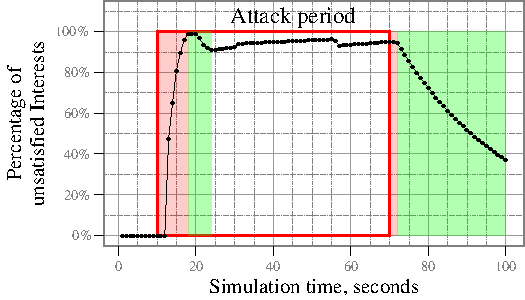
\includegraphics[scale=1]{limits}
  \caption{Dynamics of the unsatisfied Interests statistics on gateway's interface towards the attacker}
  \label{fig:ratio example}
\end{figure}


%%% Local Variables: 
%%% mode: latex
%%% TeX-master: "../paper"
%%% End: 


%%%%%%%%%%%%%%%%%%%%%%%
%%%%%%%%%%%%%%%%%%%%%%%
%%%%%%%%%%%%%%%%%%%%%%%

\subsubsection{\textbf{Probabilistic Interest accept}}
\label{sec:probabilistic}


Having successfully implemented a technique to gather statistics on Interest satisfaction ratios, our next challenge is in using this rotio to penalize malicious Interests. A straightforward method to achieve this enforcement is to use the Interest satisfaction ratio as a direct probability for accepting (forwarding) or rejecting an incoming Interest (see Pseudocode~\ref{alg:probabilistic model}).
%Apart from the Interest satisfaction statistics generation, there is a question how this statistics can be used to actually enforce prioritization and penalizing of Interests.


\floatname{algorithm}{Pseudocode}

%%%%%%%%%%%%%%%%%%%%%%%%%%%%%%
%%%%%%%%%%%%%%%%%%%%%%%%%%%%%%
%%%%%%%%%%%%%%%%%%%%%%%%%%%%%%

\begin{algorithm}[h]
\footnotesize
\caption{\small Satisfaction-based Interest acceptance}
\label{alg:probabilistic model}
\begin{algorithmic}[1]
\State{} \Comment{Same init, InData and Timeout functions as in Pseudocode~\ref{alg:queuing}}

\vspace{0.1cm}
\Function{OutInterest}{Interest \textbf{i}, InInterface \textbf{in}, OutInterface \textbf{out}}

    \State{} \Comment{Use uniform probability distribution model $P(X)$}
    \State{} \Comment{$P(X) : \forall x \in [0,1] \Rightarrow P(x) = x$}
    
    \If{$F_{in} > \theta $} \Comment{At least some Interests were forwarded before}
        \State $s \leftarrow (1 - U_{in} / F_{in})$
        \State Drop interest with probability $P(s)$
    \EndIf

    \State{forward the Interest, subjecting to token bucket limits}
\EndFunction

\end{algorithmic}
\end{algorithm}

Parameter $\theta$ on line 5 of the Pseudocode~\ref{alg:probabilistic model} ensures that the probabilistic model is not enforced when the volume of Interests arriving at a particular interface is small. This step is critical---while we want to drop Interests from attackers, we also want to provide an opportunity for legitimate users to regain their share of resources after temporary Data delivery failures due to  congestion.

A drawback of the satisfaction-based Interest acceptance method is that each router on the path makes an independent decision on whether to forward or drop the Interest. 
As a result of these independent decisions,  the probability of legitimate Interests being forwarded decreases rapidly as the number of hops between the content requester and producer grows; worsening the Interest satisfaction statistics and resulting in further drops.
In example on Fig.~\ref{fig:flooding example}, the router A observes 50\% satisfaction rate for \texttt{eth1} and 0\% rate for \texttt{eth0}. 
At the same time, router B observes a 30\% satisfaction rate for its \texttt{eth0} interface.
Next time a legitimate Interest arrives at router A, it has a 50\% chance of being forwarded further, and if forwarded, it has only a $50\% \times 30\% = 15\%$ probability of being forwarded further towards the Data producer. With each increasing hop in the network, the probability of being forwarded to the next hop decreases significantly. 
One way to prevent this overreaction and unfair penalization is to ensure that the decision taken at each router on whether to forward or drop the Interest is not independent of the decision taken at preceding routers. An explicit notification such as a gossip protocol between neighboring NDN routers that specifies the volume of Interests each router is willing to forward will likely address this issue. We leave the implementation and evaluation of a gossip protocol to future work.
%{\color{red}Alex: we should state that it is out of scope of the paper to evaluate this issue}

%%% Local Variables: 
%%% mode: latex
%%% TeX-master: "../paper"
%%% End: 


%%%%%%%%%%%%%%%%%%%%%%%
%%%%%%%%%%%%%%%%%%%%%%%
%%%%%%%%%%%%%%%%%%%%%%%

\subsubsection{\textbf{Dynamic adjustments of window-based limits}}
\label{sec:dynamic limits}


% Differential treatment of Interests received from different interfaces can be achieved in a more elegant way, without reverting to probabilistic methods.

Essentially, the probabilistic Interest accept algorithm divides the available forwarding tokens between interfaces proportionally to their satisfaction ratios.
Exactly the same effect can be achieved without using probabilistic methods, simply by enabling and enforcing additional Interest limits for each incoming interface, where the values of the limits directly depend on the interface satisfaction ratios.
Additionally, routers may need to explicitly announce these limits to their downstream neighbors, ensuring that any forwarded Interest from the downstream is actually getting through, resulting in genuine Interest satisfaction statistics.

The formal definition of the dynamic limits algorithm is presented in Pseudocode~\ref{alg:dynamic limits}, while Fig.~\ref{fig:dynamic limits example} illustrates how the algorithm would work in our toy example on Fig.~\ref{fig:flooding example}.
Assuming the initial (physical) limit $L=10$ and the current satisfaction ratios on the the router A are 50\% for \texttt{eth1} and 0\% for \texttt{eth0}, and on the router B the ratio is 30\%  \texttt{eth0}, each node would set and announce the following  incoming interface limits $L'$: 
\begin{enumerate}
\item the router B would set and announce the incoming interface limit $L'=3$;
\item the router A, after receiving announcement from B would readjust its incoming interface limits to $L'_{eth1} = 1.5$ and $L'_{eth0} = 0$; and
\item legitimate user and adversary may either obey or ignore the announced limit, which will be in any case enforced by the router A.
\end{enumerate}


\begin{figure}[htbp]
  \centering
  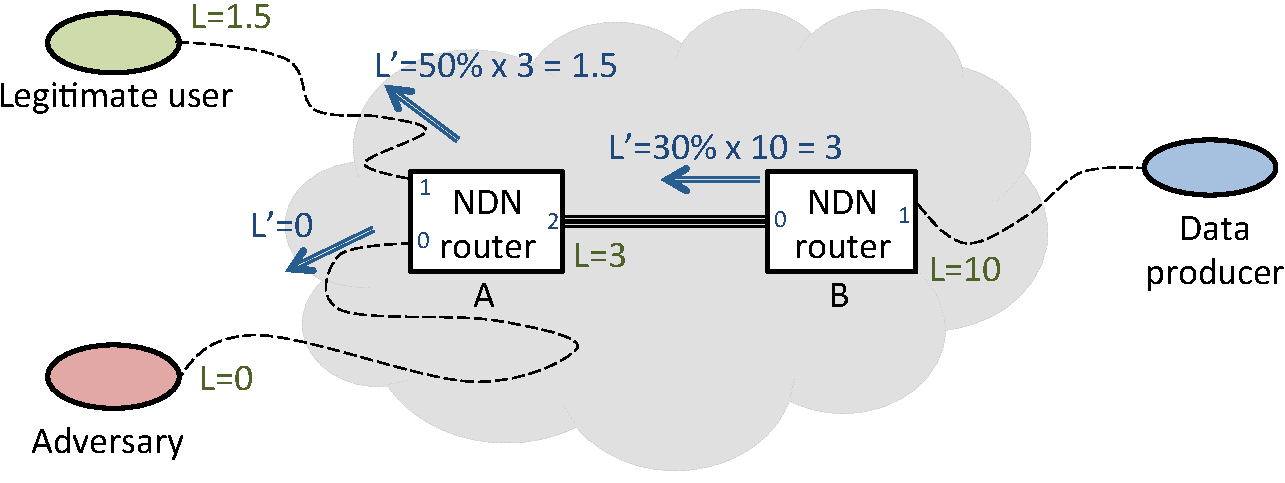
\includegraphics[width=\columnwidth]{dynamic-limits}
  \caption{Dynamic limits example: routers explicitly tell neighbors how many Interest can be for sure delivered to the Data producer}
  \label{fig:dynamic limits example}
\end{figure}


\floatname{algorithm}{Pseudocode}

%%%%%%%%%%%%%%%%%%%%%%%%%%%%%%
%%%%%%%%%%%%%%%%%%%%%%%%%%%%%%
%%%%%%%%%%%%%%%%%%%%%%%%%%%%%%

\begin{algorithm}[h]
\caption{Dynamic limits}
\label{alg:dynamic limits}
\begin{algorithmic}[1]
\State{} \Comment{Same initialization, InData and Timeout functions as in Physical Limits algorithm}
\vspace{0.2cm}
\State{$\forall f \in \mathrm{interfaces} : L'_{f} \leftarrow L_{f}$} \Comment{Per-incoming interface Interest limit} 

\vspace{0.2cm}

\State{} \Comment{\textit{Announcement from the neighbor}}
\Function{InLimits}{InInterface $if$, Limit $L'$}
    \State $L_{if} \leftarrow L'$
\EndFunction

\vspace{0.2cm}

\Function{AnnounceLimits}{} \Comment{\textit{E.g., every second}}
\For{\textbf{each} outgoing interface $of$}

   \For{\textbf{each} incoming interface $if$}
        \State $L'_{if}= {L_{of}} \times (1 - U_{if}/F_{if})$
        \State AnnounceLimit($if$, $L'_{if}$)
   \EndFor

\EndFor
\EndFunction

\end{algorithmic}
\end{algorithm}

The zero limit for the adversary's link means that the router A is temporarily not willing to accept any interests from this link, not until the statistics decays to the appropriate level (recall Fig.~\ref{fig:ratio example}).
At the next iterations of the dynamic limits algorithm, the legitimate user will be able to gradually improve the statistics on both the router A and router B (all his Interests will get through and will return Data), eventually resulting in a full allowance ($L'=L=10$) in the links between the routers A and B, and the user and the router A.

It should be noted that while in the description of the dynamic limits algorithm we used notions of ``outgoing'' and ``incoming'' interfaces, in the real system all interfaces can be both incoming and outgoing.
Thus, it may not be entirely clear which outgoing limit $L_{of}$ (line 10 in the algorithm) should be used to calculate the incoming limit $L_{if}$.
To overcome this problem, in our actual implementation we enforced separate incoming/outgoing interface limits for each individual FIB entry.
That is, for each FIB entry we set a separate Interest limit for each incoming interface ($L'_{{if}^{FIB}}$) based on a sum of FIB entry limits for each outgoing interface $L=\sum{L_{{of}^{FIB}}}$.


% Alex: not sure if this paragraph belongs here
Essentially, both probabilistic Interest accept and the dynamic limits algorithm are forms of a well-known push-back mechanism~\cite{Pushback}, with several core differences.
First, we are suppressing (pushing back) unwanted requests for Data, not the actual Data.
Second, differentiating between good and bad Interests is based on the traffic symmetry property of NDN.
% Alex: I'm not entirely sure about this point... 
Finally, both intelligent attack mitigation algorithms can be enabled all the time, without degrading network performance when there are no active attack.


%%% Local Variables: 
%%% mode: latex
%%% TeX-master: "../paper"
%%% End: 


%%% Local Variables: 
%%% mode: latex
%%% TeX-master: "paper"
%%% End: 
